\documentclass[11pt, twocolumn]{article}
\usepackage{graphicx}
\usepackage{url}
\usepackage{listings}
\setlength{\columnsep}{0.3in}
\usepackage[margin=1in]{geometry}
\linespread{1.05}

\author{Ian Foster, Jon Larson, and Max Masich}
\title{A Study of SMTP [in]Security}
\date{}

\begin{document}
\maketitle

\begin{abstract}
The Simple Mail Transfer Protocol (SMTP) and related Extended SMTP (ESMTP) are 
the primary means of delivering email messages between servers over the internet 
today.  Internet traffic can easily be collected by third-parties, yet 
encryption of SMTP messages is not universal, and in fact cannot be required by 
a Mail Exchange (MX) server.  This means that it is possible for an inter-domain 
email to be transferred and/or stored as plain-text at at least one point on its 
path across the internet.  This paper provides an analysis of current email 
providers and their support for TLS encryption over SMTP.  We show that while a 
majority of SMTP servers do provide support for TLS, almost half of all email 
users use a provider that does not support TLS encryption according to the 
standard ESMTP protocol.  We further show that of those email providers that 
ostensibly support TLS, a number of them are configured such that their true 
security is suspect (e.g. invalid certificates, weak ciphers).  Our aim is to 
raise awareness of the vulnerabilities present in the current SMTP environment
on the internet.
\end{abstract}

\section{Introduction}


\section{Background}
As the ARPANET grew throughout the 1970s, researchers started designing ways of sending messages to other users on remote hosts, using already standardized protocols such as FTP.  By 1979, there were already a myriad of incompatible standards, and researchers began to devise a unified standard for transferring mail (RFC 808).  In 1981, the Simple Mail Transfer protocol was first proposed in RFC 788, and later standardized in RFC 821. However, these early versions of SMTP did not include any support for encryption. It wasn't until 1995 that Extended SMTP (ESMTP) was standardized, which allowed for arbitrary extensions to the base SMTP protocol, including the support of TLS for SMTP (RFC 2487).  Even with the addition of TLS support, SMTP servers are still not allowed to require encryption so that they can be backward-compatible.

Today, the basic process of sending an email is the following: the sending client submits a message to a Mail Submission Agent (MSA), which sends the message to a Mail Transfer Agent (MTA).  The MTA issues a DNS query to get the Mail Exchange (MX) records of the destination address, and sends the message to this server.  From there, the message is relayed (possibly using multiple MX record queries and forwards) to a Mail Delivery Agent (MDA).  Finally, the MDA delivers the message to the destination client.  It is important to note that both submission and delivery (Sender to MSA and MDA to Recipient) may use a number of different protocols, including HTTP and SMTP (on port 587) for submission and POP3 and IMAP for delivery.  However, the transfer from MTA to MX server is always done using SMTP on port 25.


\section{Related Works}
From what we could find, there has been no similar work done specifically 
studying the state of security of the SMTP ecosystem. 

On the other hand, there have been studies of a similar vein on the state HTTPS. 
One in particular that we drew inspiration from was \cite{https} in our analysis 
of SMTP TLS certificate validity. 

\section{Methodology}
\subsection{Collecting User Distributions}
In order to determine user distribution of popular email providers we acquired user leaks from Sony, having 20,000 records from 2011[], Gawker having 500,000 records from 2010[], and Adobe having 141 Million records from 2013[3]. From these leaks we would get a good idea of what mail providers were popular, and the approximate user distributions among them. It should be noted that our three data sources may be biased towards a U.S. users distribution.

\subsection{Scanning SMTP Servers}
Lists of domains were collected from the above mentioned user leaks, The Alexa Top Million Sites Index[1], and some of the DNS root zone files. For each domain we performed a DNS query for its MX records, and then for all of the MX record’s IP addresses. If no MX records are found for a domain we use the domain as it’s own MX record.. (For the purposes of this study we only collected IPv4 A records due to the fact that Ipv6 AAAA adoption for email is minimal and out testing machine did not have IPv6 connectivity.)

We also performed round robin on publicly available DNS servers to prevent rate limiting.

For every domain’s mail server’s IPs we collected the following information:
\begin{itemize}
    \item ESMTP Support
    \item TLS Support
    \item SSL Cipher Used
    \item SSL Cipher Bits
    \item The SSL Certificate provided by the server
\end{itemize}

Due to much of the scanning process being slowed down waiting for servers to respond due to network latency, we parallelized the SMTP scanning process. When running with 128 parallel requests we were able collect data for an average of 40 domains per second.

All data collected was put into a relational sqlite3 database for analysis.

\subsection{Collecting Email SMTP Headers}
After collecting security data on the SMTP servers of one million email providers and domain names, we attempted to determine what security measures were actually implemented when sending inter-domain emails among the top email providers.  To this end, we acquired accounts at seven of the top providers (outlook.com, gmail.com, yahoo.com, aol.com, web.de, gmx.de, mail.ru).  We had hoped to sign up for more accounts, but met barriers both financial (e.g. needing to pay for internet service for a comcast.net account) and geographical (e.g. needing a Chinese cell phone number to sign up for a qq.com account).

We then sent an email from each account to each of the other accounts and examined the SMTP headers, in particular the “Received” fields.  These fields are added to the header upon receipt at each server, showing the sender and receiver as well as the protocol and security measures used in the transfer.  For example, the following field from the header of an email sent from gmx.de to aol.com shows that TLSv1 encryption was used:

\begin{verbatim}
Received: from mout.gmx.net (mout.gmx.net [212.227.15.19])
  (using TLSv1 with cipher DHE-RSA-AES128-SHA (128/128 bits))
  (No client certificate requested)
  by mtain-dk12.r1000.mx.aol.com (Internet Inbound) with ESMTPS
  id 264DF38000098 for <username@aol.com>; Tue, 18 Mar 2014 20:58:36 -0400 (EDT)
\end{verbatim}

Based on these headers, we could see which pairs of providers use encryption when sending inter-domain emails.


\section{Results}
\subsection{Top Providers}
Analyzing the number of occurrences of each domain name in the Adobe and Gawker 
email leaks gave us an idea of how many users use each provider.  The ordering 
and the exact numbers of the top domains differ somewhat, but there is some 
agreement between them.  For example, six of the top ten domains are the same 
for both sources (hotmail.com, gmail.com, yahoo.com, aol.com, comcast.net, and 
mail.ru).  For each of the top providers, we ran our scanner as outline 
above.  The results are summarized in the tables \ref{table:adobe} and 
\ref{table:gawker}.

The two most striking results from these tables are that the majority of users 
(\textgreater60\%) get service from just twenty email providers, and that at least half of 
the top email providers don’t provide any support for TLS when receiving emails.  
The biggest offender appears to be hotmail.com, which also hosts the MX servers 
for a number of other very large domains (e.g. hotmail.fr, outlook.com, msn.com, 
live.com).

\begin{table}
    \caption{Adobe Leak}
    \centering
    \label{table:adobe}
    \begin{tabular}{|l|l|l|l|}
        \hline
        Domain & \% Users & ESMTP & TLS \\
        \hline
        hotmail.com & \textgreater21.36 & Yes & No \\
        gmail.com & \textgreater15.76 & Yes & Yes \\
        yahoo.com & \textgreater11.69 & Yes & Yes \\
        aol.com & 2.28 & Yes & Yes \\
        comcast.net & 0.82 & Yes & No \\
        mail.ru & 0.82 & Yes & No \\
        web.de & 0.8 & Yes & Yes \\
        qq.com & 0.63 & Yes & No \\
        gmx.de & 0.63 & Yes & Yes \\
        naver.com & 0.43 & Yes & No \\
        \hline
    \end{tabular}
\end{table}

\begin{table}
    \caption{Gawker Leak}
    \centering
    \label{table:gawker}
    \begin{tabular}{|l|l|l|l|}
        \hline
        Domain & \% Users & ESMTP & TLS \\
        \hline
            gmail.com & \textgreater32.24 & Yes & Yes \\
            yahoo.com & \textgreater20.46 & Yes & Yes \\
            hotmail.com & \textgreater15.66 & Yes & No \\
            aol.com & 3.81 & Yes & Yes \\
            comcast.net & 1.5 & Yes & No \\
            mac.com & 1.08 & Yes & No \\
            verizon.net & 0.47 & Yes & No \\
            cox.net & 0.41 & Yes & No \\
            earthlink.net & 0.38 & Yes & No \\
            mail.ru & 0.3 & Yes & No \\
            naver.com & 0.43 & Yes & No \\
        \hline
    \end{tabular}
\end{table}

\subsection{TLS Support}
We first looked at just the proportion of email providers that support the 
STARTTLS command, ranked in order of number of users (as found in the Adobe 
leak).  We already know from table \ref{table:adobe} that of the top 10, only 
50\% support TLS.  As can be seen in figure \ref{server_tls}, of the top 2000 providers, 
only 47.94\% support TLS.  We were surprised to see, however, that support for 
TLS actually increases as we looked at more and more providers, such that of the 
top 20,000 providers, 57.63\% supported TLS, and at 100,000 the number leveled 
off around 62.75\%.  We’re not entirely sure why we see this result, but one 
possible explanation is that many smaller, less-used email providers use Google 
mail servers, which support TLS, instead of setting up their own.

\begin{figure}
    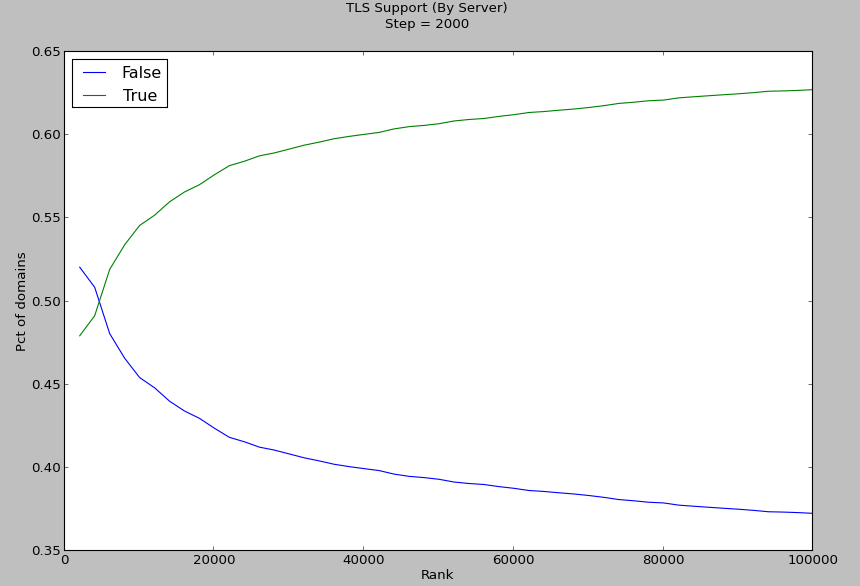
\includegraphics[width=3.0in]{images/server_tls.png}
    \caption{TLS Support by Server}
    \label{server_tls}
\end{figure}

\begin{figure}
    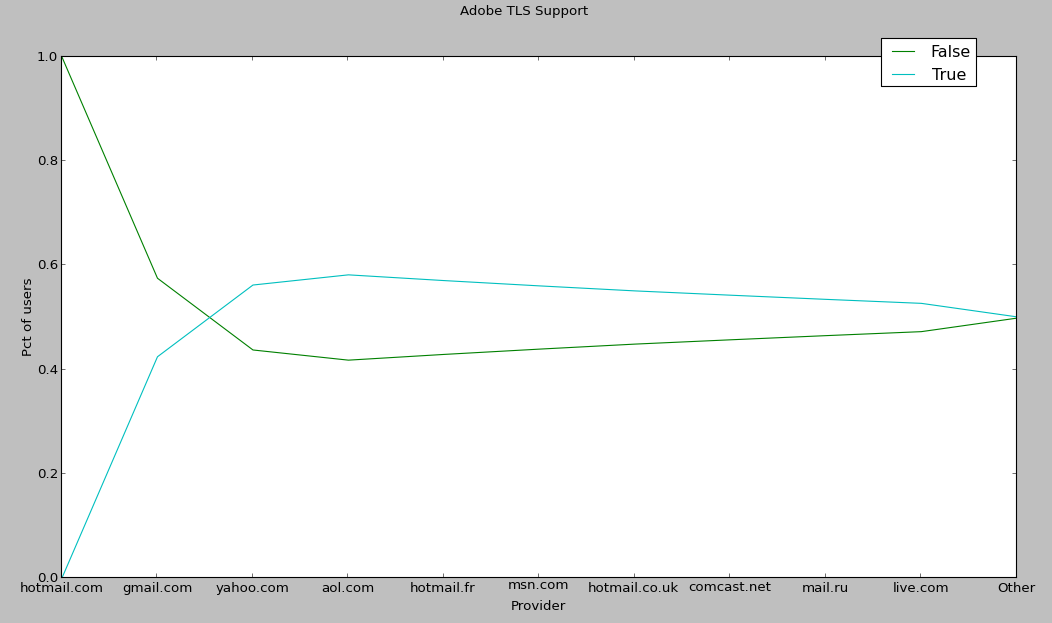
\includegraphics[width=3.0in]{images/adobe_tls.png}
    \caption{Adobe TLS Support}
    \label{adobe_tls}
\end{figure}

\begin{figure}
    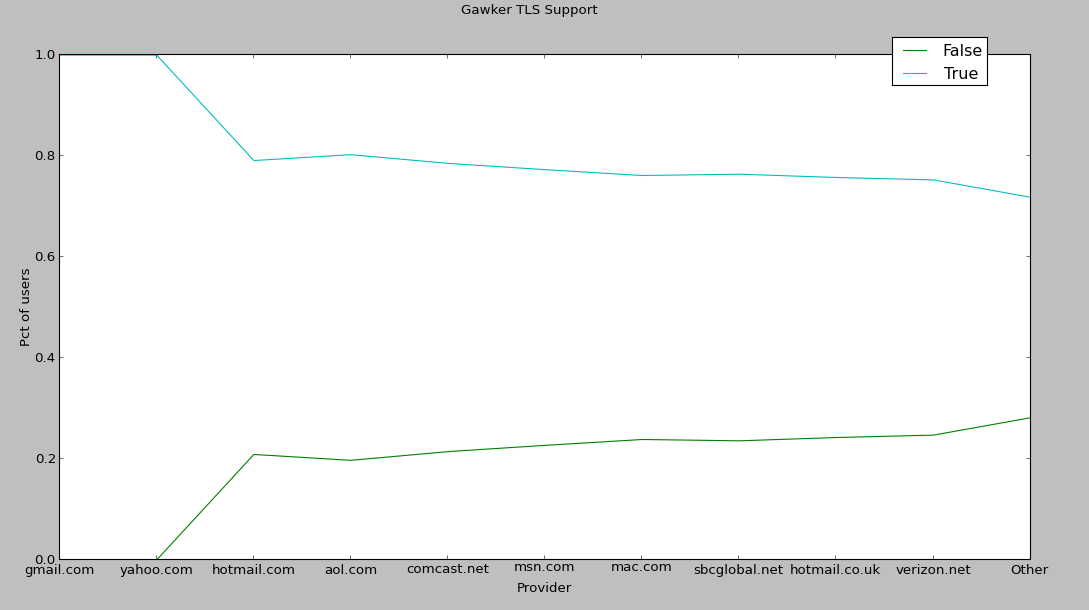
\includegraphics[width=3.0in]{images/gawker_tls.png}
    \caption{Gawker TLS Support}
    \label{gawker_tls}
\end{figure}

When we look at the proportion of actual users that have TLS support, however, 
the numbers are not quite as positive.  Looking at just the top 10 providers in
the Adobe leak (\ref{adobe_tls}), only 52.72\% of users have a provider that supports TLS, and
looking at our whole dataset that number goes down to 50.13\%.  That would
suggest that of all the email users (at least, the ones who register with Adobe),
only half receive emails with any encryption.  The numbers derived from the
Gawker leak (\ref{gawker_tls}) are considerably better (75.28\% for top 10, 71.84\% support for all
providers) but again, we consider this source to be less representative of an
international user base and more of an American (or at least Anglophone) user
base.  In either case, this still implies that at most about 72\% of email users
receive encrypted emails.

\subsection{Valid Encryption}
Based on the results of the previous section, we know that about 62\% of domains 
(covering between 50\% and 72\% of users) ostensibly support TLS, but we wanted to 
determine if those connections were really secure.  To do this, we opened secure 
connections to the SMTP servers and collected security certificates and cipher 
information.  Of the providers that support TLS, we found that only 75.9\% of 
them have valid certificates (i.e. they were signed by a trusted CA).  However, 
when looking at the proportion of users who use those providers, the numbers are 
much more positive: according to the Adobe leak, 98\% of users that use TLS have 
valid certificates, and according to the Gawker leak, 99.44\% use valid 
certificates.

We also examined the types of ciphers being used by providers who support TLS to 
see if many were using algorithms with known weaknesses. We found eleven ciphers 
used by the servers in our study; figure \ref{cipher_pie}. The only ciphers found that 
have known weaknesses are RC4-MD5 and RC4-SHA, together they are used by less 
than 0.06\% of the servers in this study.

\begin{figure}
    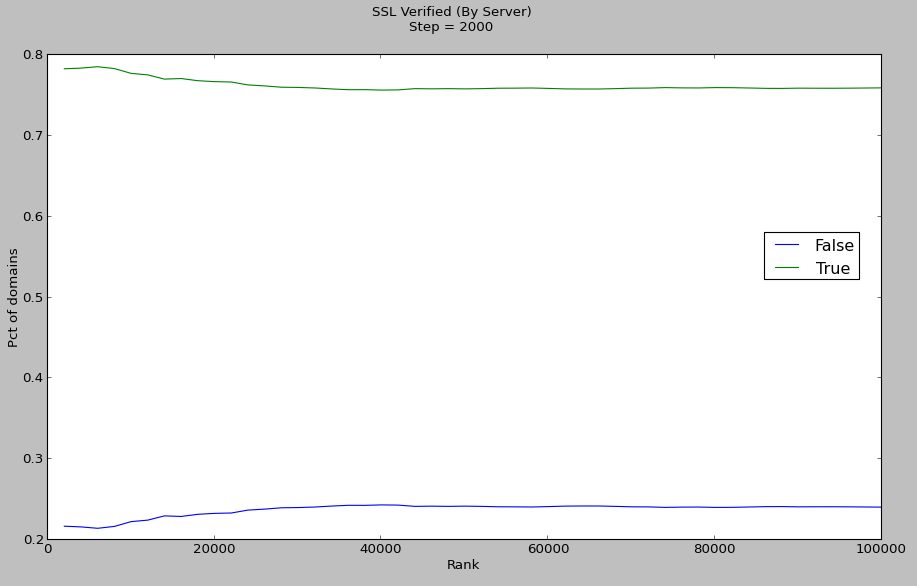
\includegraphics[width=3.0in]{images/server_verified.png}
    \caption{Valid SSL Cert by Server}
    \label{server_verified}
\end{figure}

\begin{figure}
    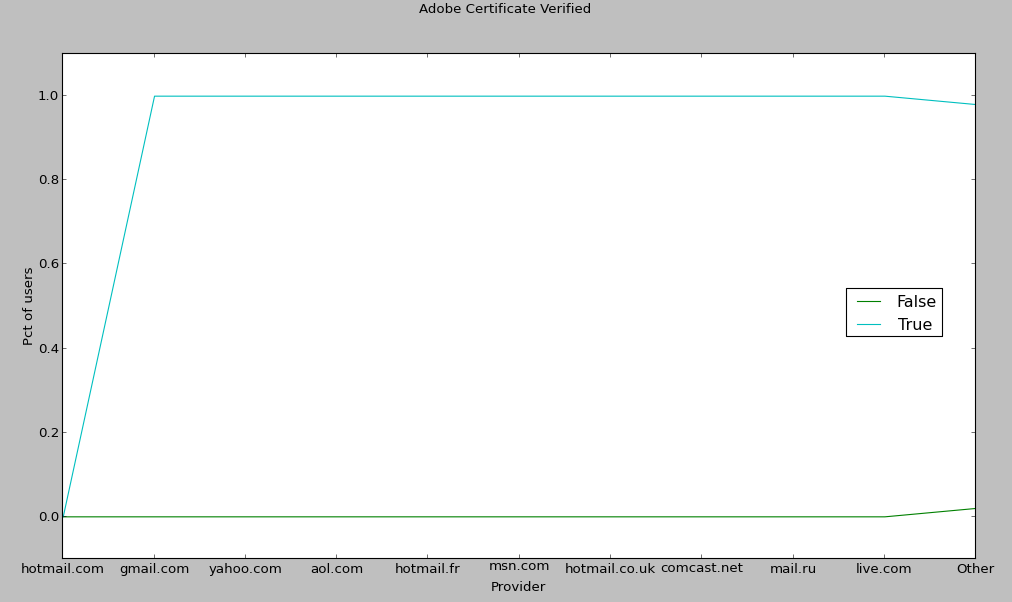
\includegraphics[width=3.0in]{images/adobe_verified.png}
    \caption{Adobe Valid Cert}
    \label{adobe_verified}
\end{figure}

\begin{figure}
    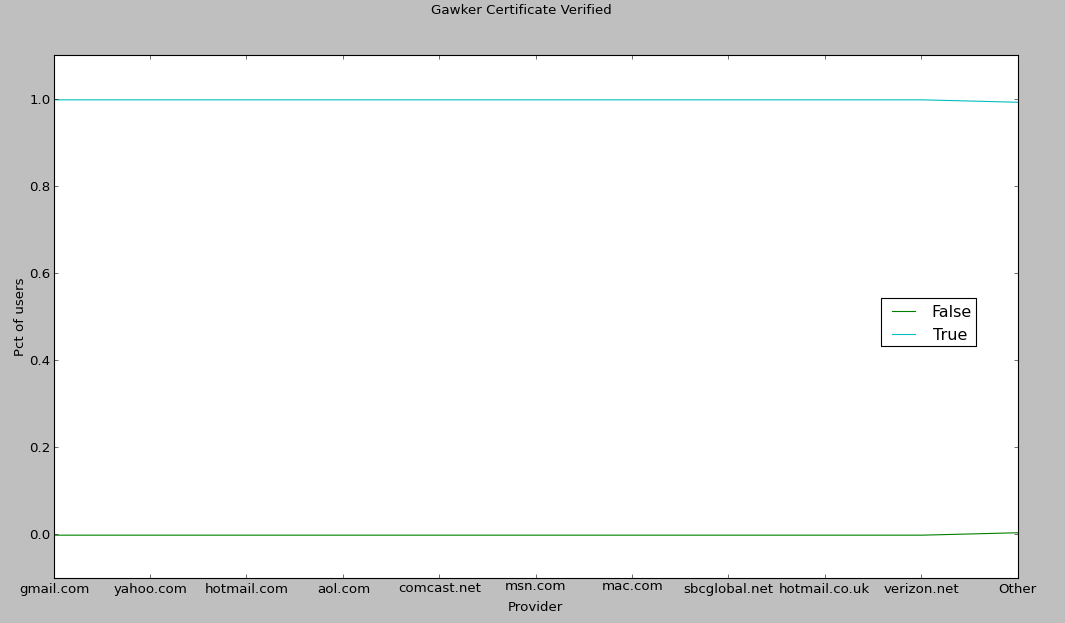
\includegraphics[width=3.0in]{images/gawker_verified.png}
    \caption{Gawker Valid Cert}
    \label{gawker_verified}
\end{figure}

\begin{figure}
    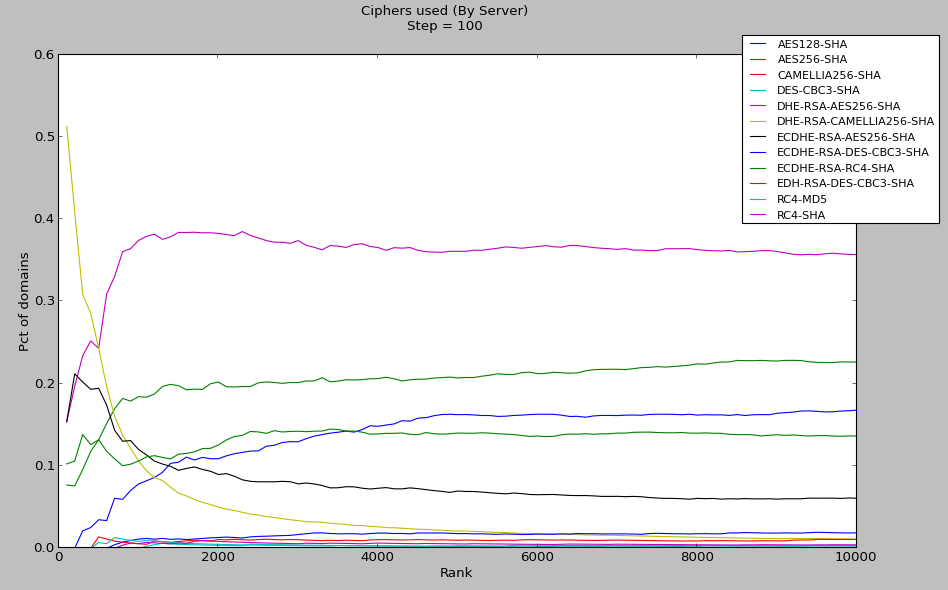
\includegraphics[width=3.0in]{images/server_ciphers.png}
    \caption{Cipher by Server}
    \label{server_ciphers}
\end{figure}

\begin{figure}
    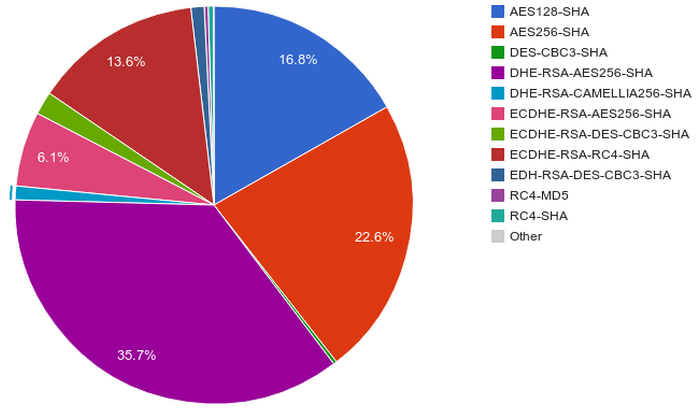
\includegraphics[width=3.0in]{images/pie_ciphers.png}
    \caption{Cipher Pie (Yum!)}
    \label{cipher_pie}
\end{figure}

\subsection{Overall Findings}
When looking at the ESMTP, TLS, and certificates use among all of the top 
million email providers Figure \ref{overall} we find that almost all 
providers support ESMTP with an adoption rate of 99.29\%. TLS support is only 
found on just over half of the providers at 54.58\%. Only 42.45\% of all 
providers, or 77.84\% of the providers with TLS, have a valid SSL 
certificate.

\begin{figure}
    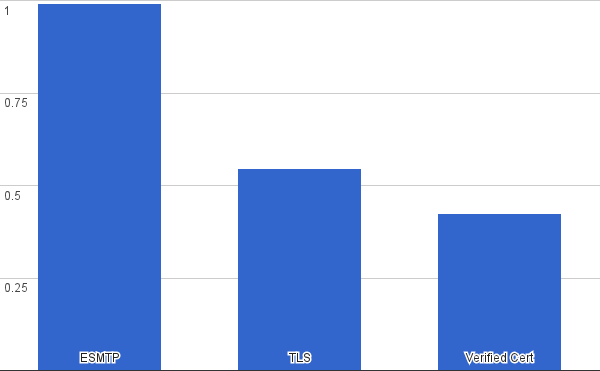
\includegraphics[width=3.0in]{images/bar_overall.png}
    \caption{TLS Adoption by Domain}
    \label{overall}
\end{figure}

\subsection{Analysis of SMTP Headers}
After determining the state of security for one million email domains, we 
examined what effect that actually has when sending emails between domains by 
tracing the Received field of SMTP headers.  The results can be seen for seven 
of the top ten email providers in Figure \ref{email_analysis}, which shows the sender and 
receiver domains along with the protocol/encryption information for the 
inter-domain hop of the message.  Of those seven, all but hotmail.com and 
mail.ru support TLS.

\begin{figure*}
    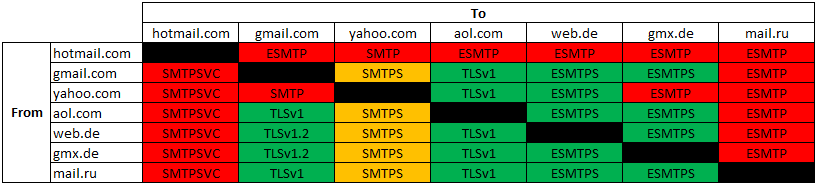
\includegraphics[width=6.0in]{images/email_analysis.png}
    \caption{SMTP Headers}
    \label{email_analysis}
\end{figure*}

The most obvious result is that the domains that do not support the STARTTLS 
command do not receive messages with encryption, which was to be expected.  A 
somewhat surprising result was that hotmail.com, which does not support TLS on 
incoming emails, also does not use TLS on its outgoing emails.  However, mail.ru 
uses the encryption settings of the destination server, even though it does not 
use encryption on incoming emails.  An even more surprising discovery was that 
yahoo.com did not use encryption when sending to gmail.com or gmx.de, even 
though all three domains support TLS.

We were somewhat unsure as to the level of encryption provided on emails bound 
for yahoo.com.  Headers with explicit cipher information were obviously sent 
with encryption, and IANA defines the ESMTPS parameter as indicating ESMTP 
with STARTTLS\cite{mail}. We assume that SMTPS similarly indicates that STARTTLS (or some other 
encryption mechanism) was used, but there is no official SMTPS parameter.

The implication of these results is that, while approximately 60\% of domains 
support TLS on incoming messages, not all MTAs actually make use of it when 
sending to those servers.  It is impossible to tell just what percent of 
email traffic is unencrypted without looking at the actual numbers of emails 
moving between different domains.  However, if only 50\% of users are on 
providers that support TLS on incoming messages and not all domains actually 
make use of that encryption when sending to those providers, it is 
reasonable to assume that at most 50\% of users are actively using 
encryption, and the number is probably somewhat lower.

\subsection{Outsourced Mail}
Many of the top domains actually share a common set of SMTP servers. This is due 
to providers such as Google and Microsoft who host email for domains owned by 
other companies. When we looked at who hosted the email of the top million 
providers we saw that the majority of email was being hosted by the five 
companies listed in table \ref{table:top_servers}. Here we see that Google hosts 
the most with 11\% of the domains email. The values listed in table 
\ref{table:top_servers} represent the lower bound of the amount of domains each 
provider is in control of.

\begin{table}
    \caption{Top Mail Servers by Domain}
    \centering
    \label{table:top_servers}
    \begin{tabular}{|l|l|}
        \hline
        Provider & \% of Domains \\
        \hline
        Google & 11.03\% \\
        Microsoft & 3.45\% \\ 
        GoDaddy & 2.06\% \\
        MX Logic & 1.58\% \\
        RackSpace & 1.32\% \\
        \hline
    \end{tabular}
\end{table}


\section{Future Work}
Due to the time constraints of this project only a small sample of a few million 
domains, a larger sample of the entire internet, especially if ranked by region 
could provide good insight into that state of secure email communication on an 
country by country basis.

A follow up study collecting the same data would allow us to see how the 
adoption of TLS for SMTP is changing.

In addition to TLS, SMTP can also make use of Sender Policy Framework (SPF) 
records for authentication of email origin, and DomainKeys Identified Mail 
(DKIM) to verify message integrity. Our study could benefit further by checking 
for the usage of SPF and DKIM use coverage.  

Determine reason for Microsoft not supporting TLS. In our preliminary 
investigation, it was unclear why they would not even support the option for 
other services to send with TLS. Ideally, we would like to get in touch of 
the hotmail team to see if we can get an answer to this question directly.

Explore alternatives to SMTP for email communication. An ideal mail protocol 
would provide end-to-end email encryption. Not only would such a protocol 
provide stronger data security and integrity, but it could also have the 
potential for alleviating spam. 

Many online services send automated emails that may contain sensitive 
information such as clear text passwords, password reset links, order 
information, etc, which may not be sent via the same route as non-automated 
email from that domain. An analysis of automated email headers from popular 
providers would give us insight into this issue.

\section{Conclusion}


\begin{thebibliography}{1}
    \bibitem{alexa}
        Alexa Top 1,000,000 Sites

        \url{http://www.alexa.com/topsites/global}
    \bibitem{https}
        Analysis of the HTTPS Certificate Ecosystem

        \url{http://web.eecs.umich.edu/~mibailey/publications/imc13\_https\_final.pdf}
    \bibitem{adobe}
        Adobe Email Leak

        \url{http://www.theguardian.com/technology/2013/nov/07/adobe-password-leak-can-check}
    \bibitem{gawker}
        Gawker Email Leak

        \url{http://www.slate.com/articles/technology/technology/2010/12/was\_your\_gawker\_password\_hacked.html}
    \bibitem{sony}
        Sony Email Leak
    \bibitem{821}
        RFC 821

        \url{http://tools.ietf.org/html/rfc821}
    \bibitem{2487}
        RFC 2487

        \url{http://tools.ietf.org/html/rfc2487}
    \bibitem{code}
        Project Code

        \url{https://github.com/lanrat/smtp-scanner}
    \bibitem{mail}
        Mail Parameters

        \url{http://www.iana.org/assignments/mail-parameters/mail-parameters.xhtml}
\end{thebibliography}

\end{document}
